\documentclass[tikz,border=15pt]{standalone}
\usepackage{tikz}
\usepackage{amsmath}
\usetikzlibrary{shapes.geometric,arrows.meta,positioning,calc,backgrounds,fit}

\begin{document}
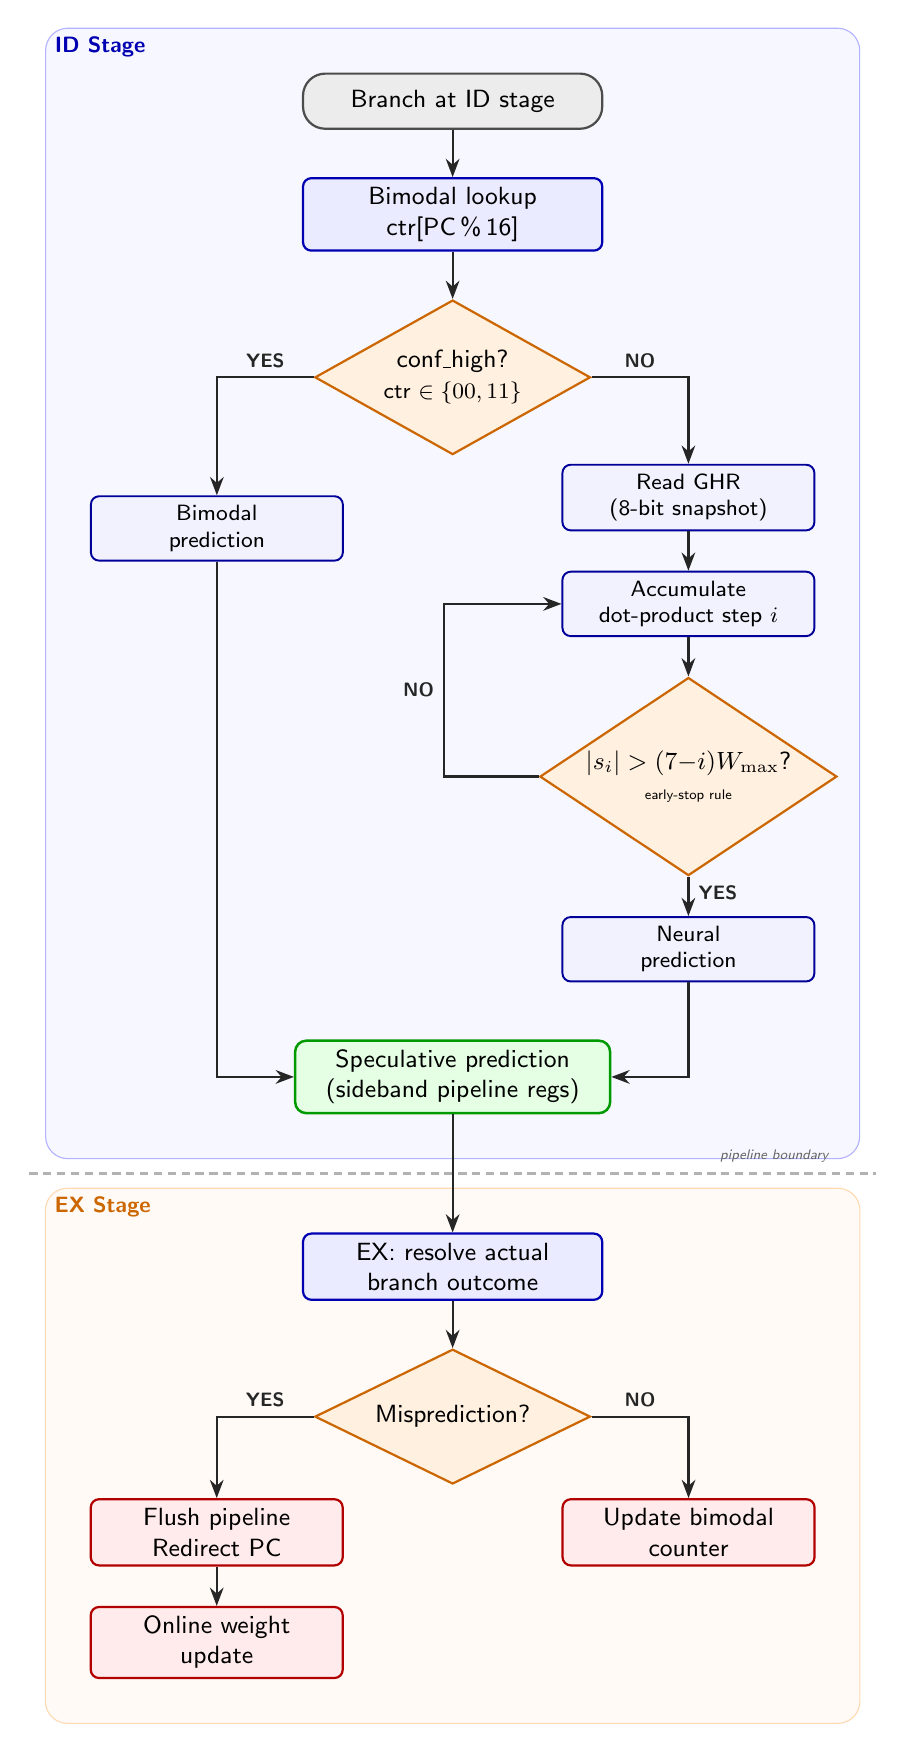
\begin{tikzpicture}[
  font=\sffamily\small,
  every node/.style={align=center},
  %% ─── 樣式定義 (模組化與視覺優化) ─────────────────────────────────
  terminal/.style={
    draw=black!70, fill=gray!15, rounded corners=8pt,
    minimum width=3.8cm, minimum height=0.7cm, line width=0.8pt},
  process/.style={
    draw=blue!70!black, fill=blue!8, rounded corners=3pt,
    minimum width=3.8cm, minimum height=0.7cm, line width=0.8pt},
  subproc/.style={
    draw=blue!60!black, fill=blue!5, rounded corners=3pt,
    minimum width=3.2cm, minimum height=0.65cm,
    font=\sffamily\footnotesize, line width=0.7pt},
  decision/.style={
    draw=orange!80!black, fill=orange!12, diamond, aspect=1.5,
    minimum width=3.5cm, minimum height=1.2cm,
    inner sep=1pt, line width=0.8pt},
  predict/.style={
    draw=green!60!black, fill=green!10, rounded corners=4pt,
    minimum width=4.0cm, minimum height=0.75cm, line width=0.9pt},
  update/.style={
    draw=red!70!black, fill=red!8, rounded corners=3pt,
    minimum width=3.2cm, minimum height=0.7cm, line width=0.8pt},
  %% ─── 箭頭與標籤樣式 ──────────────────────────────────────────
  arr/.style={->, >=Stealth, line width=0.8pt, color=black!85},
  labarr/.style={->, >=Stealth, line width=0.8pt, color=black!85}
]

  %% ════════════════════════════════════════════════════════════════
  %%  ID STAGE (主軸置中對齊，動態推導相對位置)
  %% ════════════════════════════════════════════════════════════════
  \node[terminal] (start) {Branch at ID stage};
  \node[process, below=0.6cm of start] (bimodal) {Bimodal lookup\\ctr[PC\,\%\,16]};
  \node[decision, below=0.6cm of bimodal] (conf) {\small conf\_high?\\{\footnotesize ctr $\in \{00,11\}$}};

  %% ── High-confidence path (左側分支) ──────────────────────────
  \node[subproc, below left=1.0cm and 0.5cm of conf] (bimout) {Bimodal\\prediction};

  %% ── Low-confidence path (右側神經網路分支) ────────────────────
  \node[subproc, below right=0.6cm and 0.5cm of conf] (ghr) {Read GHR\\(8-bit snapshot)};
  \node[subproc, below=0.5cm of ghr] (acc) {Accumulate\\dot-product step $i$};
  \node[decision, below=0.5cm of acc] (estop) {$|s_i|>(7{-}i)W_{\max}$?\\{\tiny early-stop rule}};
  \node[subproc, below=0.5cm of estop] (nout) {Neural\\prediction};

  %% ── Merge node ──────────────────────────────────────────────────
  % 確保 speculative prediction 節點絕對置中，且位於 nout 的正下方
  \node[predict] (pred) at (start |- nout.south) [yshift=-1.2cm] {Speculative prediction\\(sideband pipeline regs)};

  %% ════════════════════════════════════════════════════════════════
  %%  EX STAGE
  %% ════════════════════════════════════════════════════════════════
  \node[process, below=1.5cm of pred] (exres) {EX: resolve actual\\branch outcome};
  \node[decision, below=0.6cm of exres] (misp) {Misprediction?};

  %% ── YES path (左側 Flush 與 Update) ─────────────────────────
  \node[update, below left=0.6cm and 0.5cm of misp] (flush) {Flush pipeline\\Redirect PC};
  \node[update, below=0.5cm of flush] (wupd) {Online weight\\update};

  %% ── NO path (右側 Counter Update) ───────────────────────────
  \node[update, below right=0.6cm and 0.5cm of misp] (cupd) {Update bimodal\\counter};


  %% ════════════════════════════════════════════════════════════════
  %%  訊號佈線 (Routing Logic)
  %% ════════════════════════════════════════════════════════════════
  \draw[arr] (start) -- (bimodal);
  \draw[arr] (bimodal) -- (conf);

  % conf YES → left path
  \draw[labarr] (conf.west) -| node[pos=0.25, above, font=\sffamily\scriptsize\bfseries] {YES} (bimout.north);
  
  % conf NO → right path
  \draw[labarr] (conf.east) -| node[pos=0.25, above, font=\sffamily\scriptsize\bfseries] {NO} (ghr.north);

  % Right branch internal flow
  \draw[arr] (ghr) -- (acc);
  \draw[arr] (acc) -- (estop);

  % estop YES → neural output
  \draw[labarr] (estop.south) -- node[pos=0.4, right, font=\sffamily\scriptsize\bfseries] {YES} (nout.north);

  % estop NO (early-stop loop-back) -> 完美的左側繞回佈線
  \draw[labarr] (estop.west) -- ++(-1.2,0) coordinate (loop) 
                |- node[pos=0.25, left, font=\sffamily\scriptsize\bfseries] {NO} (acc.west);

  % 匯流至 Merge node
  \draw[arr] (bimout.south) |- (pred.west);
  \draw[arr] (nout.south) |- (pred.east);

  % Pipeline flow 跨界
  \draw[arr] (pred) -- (exres);
  \draw[arr] (exres) -- (misp);

  % misp YES → flush + weight update
  \draw[labarr] (misp.west) -| node[pos=0.25, above, font=\sffamily\scriptsize\bfseries] {YES} (flush.north);
  \draw[arr] (flush) -- (wupd);

  % misp NO → counter update
  \draw[labarr] (misp.east) -| node[pos=0.25, above, font=\sffamily\scriptsize\bfseries] {NO} (cupd.north);


  %% ════════════════════════════════════════════════════════════════
  %%  動態背景封裝與邊界線 (Background & Separation)
  %% ════════════════════════════════════════════════════════════════
  \begin{scope}[on background layer]
    % ID Stage 動態包覆框
    \node[draw=blue!30, fill=blue!3, rounded corners=8pt, inner sep=16pt,
          fit=(start) (bimout) (loop) (ghr) (nout) (pred)] (idbox) {};
    \node[anchor=north west, font=\sffamily\footnotesize\bfseries, text=blue!70!black] 
          at (idbox.north west) {ID Stage};

    % EX Stage 動態包覆框
    \node[draw=orange!30, fill=orange!4, rounded corners=8pt, inner sep=16pt,
          fit=(exres) (misp) (flush) (wupd) (cupd)] (exbox) {};
    \node[anchor=north west, font=\sffamily\footnotesize\bfseries, text=orange!80!black] 
          at (exbox.north west) {EX Stage};

    % 智慧型流水線邊界 (自動抓取兩方框的水平範圍並精準對分垂直空間)
    \coordinate (boundY) at ($(pred.south)!0.5!(exres.north)$);
    \draw[densely dashed, gray!60, line width=1.2pt] 
          ([xshift=-0.2cm]idbox.west |- boundY) -- ([xshift=0.2cm]idbox.east |- boundY)
          node[pos=0.88, above, font=\sffamily\tiny\itshape, text=gray!80!black] {pipeline boundary};
  \end{scope}

\end{tikzpicture}
\end{document}